\chapter{DMA Controller}
\label{cha:DMA}

\section{Transazioni di input/output}
\label{sec:transazioniIO}

Si dice transazione di input/output il trasferimento di un blocco di dati strutturato in più trasferimenti elementari (nel nostro caso, da 8 bit). Ad ogni trasferimento, il calcolatore (1) acquisisce un blocco di dati, (2) li elabora, (3) ricomincia.
L'acquisizione può essere effettuata in tre modi: \textit{polling}, \textit{interrupt} o tramite DMAC.
Colui che si occupa di convogliare i dati dal mondo esterno alla memoria è il \textit{driver}, il quale è suddiviso in:
\begin{itemize}
\item \textit{initiator}: definisce la transazione e setta due registri importantissimi
\begin{itemize}
\item CAR: \textit{Current Adress Register}, inizializzato con $BASE$, parametro che indica dove inizia la porzione di memoria in cui andiamo a porre o prelevare i dati della nostra transizione;
\item CCR: \textit{Current Counter Register}, inizializzato con $N-1$ dove $N$ è il numero di transizioni da effettuare.
\end{itemize}
\item \textit{continuator}: esegue la transazione.
\end{itemize}

In figura \ref{fig:taskContinuator} viene mostrata la \textit{flow chart} sintetica del \textit{continuator} a \textit{polling}. Il suo gran daffare è chiedere continuamente alla periferica se è disponibile un nuovo dato, cosa che potrebbe essere sconveniente in quanto caricherebbe la CPU di un carico computazionale inutile e martellante.

\begin{figure}[!h]
\centering
\includegraphics[width=0.6\columnwidth]{img/taskContinuator}
\caption{\textit{Flow chart} sintetica del \textit{continuator} a \textit{polling}}
\label{fig:taskContinuator}
\end{figure}

Per scoprire se è presente un dato si interroga l'interfaccia: se esso viene trasferito in memoria vengono invece aggiornati i registri con
\[
\begin{gathered}
CAR=CAR+1\\
CCR=CCR-1
\end{gathered}
\]
Quando arriva l'ultimo dato (sono $N$ e CCR è inizialmente inizializzato a $N-1$), CCR sarà pari a -1 e la transazione sarà terminata.

In figura \ref{fig:periferica8} vediamo un esempio di periferica con $K=1$ (occupa $2^K=2^1=2$ byte, quello avente indirizzo basso per lo stato\footnote{Supporremo sia 80H.} e quello avente indirizzo alto per il dato vero e proprio\footnote{Supporremo sia 81H.}).

\begin{figure}[!h]
\centering
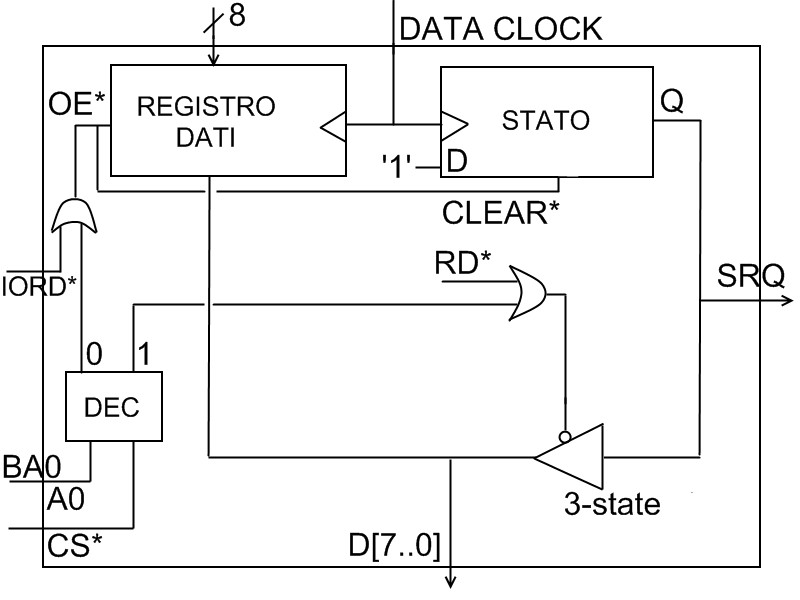
\includegraphics[width=0.65\columnwidth]{img/periferica8}
\caption{Periferica con $K=1$}
\label{fig:periferica8}
\end{figure}

Si noti che il registro di stato è un \textit{flip-flop} D che campiona il segnale '1' sul fronte positivo del cosiddetto DATA\_CLK (\textit{data clock}) che sale quando è disponibile un dato: tale registro viene resettato quando si legge il dato (segnale di CLEAR* diventa basso) e cioè quando A0 = 1 (per indirizzare 81H). 
L'uscita del \textit{flip-flop} viene detta SRQ (\textit{Service ReQuest}) e indica che vi è una transazione da compiere.
Il \textit{chip select} CS* è quello che abilita la periferica e può essere formulato usando le nozioni di Calcolatori L-A\footnote{Esempio: supponiamo di avere uno spazio di indirizzamento di 256 byte. Potrei scegliere di utilizzare gli 8 bit dell'indirizzo sfruttando la convenzione tale per cui i quattro più significativi sono quelli che selezionano la periferica, mentre gli altri quattro selezionano il dato all'interno della periferica. Facendo questa scelta abbiamo al massimo $2^4=16$ periferiche, ognuna delle quali può avere al massimo $2^4=16$ registri da 1 byte. Volendo selezionare quella che è mappata fra 80H e 8FH (8 in esadecimale = 1000) e chiamati BA7\ldots BA0 i bit di indirizzo, il \textit{chip select} sarà BA7 BA6* BA5* BA4*.}

Per quanto riguarda le tempistiche, va prestata la necessaria attenzione al fatto che:
\begin{itemize}
\item se arrivano due colpi di DATA\_CLK prima che io legga il dato, perdo quest'ultimo;
\item se resetto lo stato troppo presto, duplico il dato.
\end{itemize}

\begin{figure}[!h]
\centering
\includegraphics[width=0.75\columnwidth]{img/formeOndaPeriferiche}
\caption{Le forme d'onda dei segnali della nostra periferica}
\label{fig:formeOndaPeriferiche}
\end{figure}

\section{\textit{Polling} vs. \textit{Interrupt}}
\label{sec:pollingCriminale}

Un \textit{task} che effettua di continuo il \textit{polling} monopolizza la CPU e consuma tantissima energia. Per questo conviene svegliare la CPU solo quando arrivano i dati ed è una buona scelta mandare l'SRQ direttamente all'8254 (PIC).

\begin{figure}[!h]
\centering
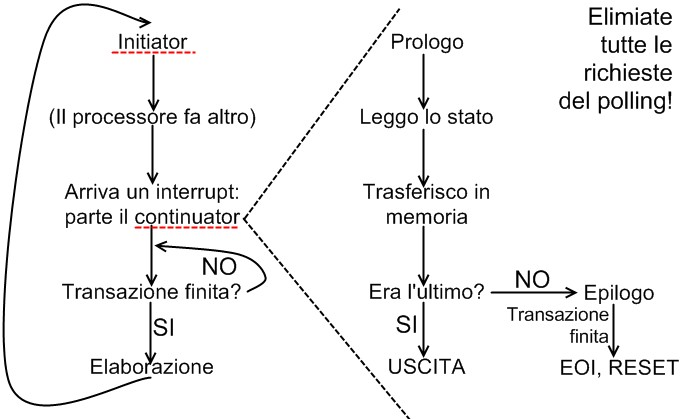
\includegraphics[width=0.75\columnwidth]{img/interrupt}
\caption{Gestione delle transazioni tramite interrupt}
\label{fig:interrupt}
\end{figure}

In figura vediamo come viene implementata la scelta di fare uso degli interrupt\footnote{Il \textit{prologo} consiste nel salvare lo stato del programma interrotto dall'\textit{interrupt}. Tale stato viene riabilitato in seguito alla fase di \textit{epilogo}.}. Si noti che la variabile \textit{transazione finita} è condivisa fra il\textit{ main program} e il \textit{continuator}.

\section{DMA}
\label{sec:DMAPOWA}

\begin{figure}[!h]
\centering
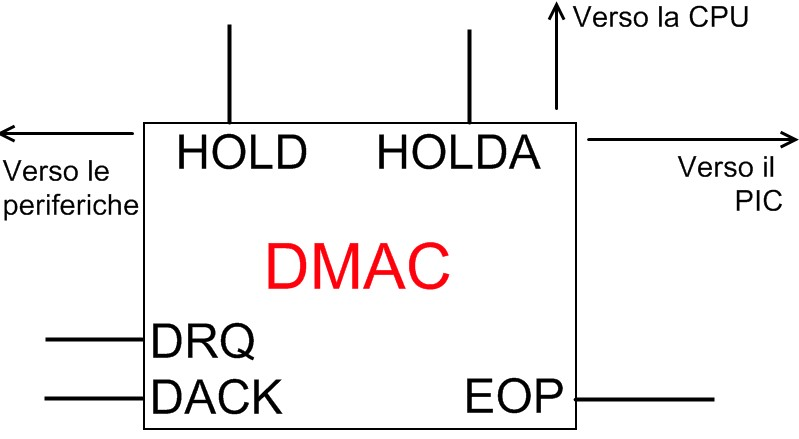
\includegraphics[width=0.534579\columnwidth]{img/DMAC}
\caption{DMA Controller, molto schematicamente}
\label{fig:DMAC}
\end{figure}

La gestione ad \textit{interrupt} è molto più \textit{smart} di quella a \textit{polling}, ma si è storicamente cercato un modo per svincolare un po' la CPU dal peso di tutte le computazioni che deve gestire: per questo è stato inventato il componente 8237 (DMAC, vedi fig. \ref{fig:DMAC}), che si prende cura di prendere i dati dalle periferiche e di mandarli in memoria senza interpellare il processore. Per poter svolgere questa funzione, ed essendo in grado di gestire fino a 4 periferiche, il DMAC possiede 4 registri CAR, 4 registri CCR e un registro MASK, settato dall'\textit{initiator}, che indica quali fra i canali collegati alle periferiche sono mascherati e quali no.

\begin{figure}[!h]
\centering
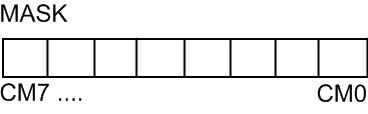
\includegraphics[width=0.45\columnwidth]{img/mask}
\caption{Registro mask}
\label{fig:mask}
\end{figure}

Come si nota in figura \ref{fig:DMAC}, il DMAC ha diversi piedini:
\begin{itemize}
\item il piedino DRQ (DMA ReQuest) e il piedino DACK: servono a gestire le richieste da parte della periferica e a interloquire con quest'ultima;
\item i piedini HOLD e HOLDA: servono a comunicare alla CPU che il DMAC vuole effettuare una transizione, in modo che non vi siano conflitti sul bus (HOLD = "'CPU, trattieniti dall'usare il bus!'");
\item il piedino EOP: il DMAC si interfaccia col PIC per gestire il corretto trattamento degli \textit{interrupt}. Quando infatti il registro CCR arriva a -1 (segno che la transazione è terminata) è necessario che il DMAC disabiliti la seriale\footnote{Altrimenti c'è il rischio che il DMAC scriva in zone di memoria che non gli competono all'interno di quella particolare transizione.} agendo sul registro MASK. Infine, viene posto ad 1 il piedino EOP, in modo che arrivi un impulso al PIC (il quale a sua volta lo girerà alla CPU): associato a questo tipo di interrupt vi è un \textit{task gate} che si occupa di far ripartire la procedura mostrata in figura \ref{fig:interrupt}.
\end{itemize} 

Grazie a queste scelte, il DMAC solleva la CPU da tutto il carico del \textit{continuator}: a questo punto essa deve semplicemente chiamare l'\textit{initiator} e poi fermarsi. Peraltro il DMAC è velocissimo in quanto effettua cicli \textit{fly-by}, ovvero legge dalle periferiche e scrive in memoria in un unico ciclo di bus. L'incremento prestazionale ottenuto con la gestione ad \textit{interrupt} risulta oltremodo evidente se consideriamo che con $N$ cicli del DMAC (1 per dato, per un totale di $N$ dati da trasferire) otteniamo lo stesso risultato che avremmo avuto coi $KN$ cicli della CPU necessari a gestire lo stesso trasferimento a \textit{polling}. 
Inoltre, volendo trasferire $N$ blocchi da $M$ byte, $NM$ operazioni del DMAC provocano solo $N$ \textit{interrupt} verso la CPU: questo significa che il DMAC divide per $M$ il carico delle richieste (vedi paragrafo \ref{sec:sequenzaDMA} per maggiori dettagli).
Il DMAC è quindi un acceleratore della CPU e lavora in modalità \textit{cycle-stealing} ("'ruba'" cicli alla CPU, sollevandola da un eccessivo carico computazionale).

\section{La sequenza degli eventi scatenati dal DMA}
\label{sec:sequenzaDMA}

\begin{figure}[!h]
\centering
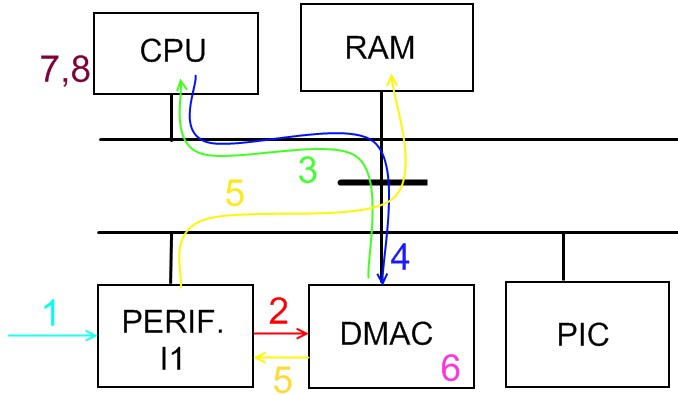
\includegraphics[width=0.75\columnwidth]{img/sequenzaEventi}
\caption{La sequenza degli eventi nel trasferimento DMAC}
\label{fig:sequenzaEventi}
\end{figure}

\begin{itemize}
\item Arriva una richiesta dalla periferica e l'interfaccia setta l'SRQ. Viene abilitato il relativo canale nel vettore MASK e vengono posti $CCR=N-1$ e $CAR=BASE$.
\item L'interfaccia gira la richiesta al DMAC.
\item Il DMAC chiede alla CPU di lasciare il BUS (\textit{Hold Request} = HRQ). La CPU finisce quel che deve finire e poi acconsente a questa richiesta.
\item La CPU dà l'OK con un \textit{hold acknowledge}. Il DMAC è ora padrone del campo e tutti i segnali di comando diventano flottanti\footnote{Si comprende allora la necessità di un \textit{pull-up} in grado di portarli al livello logico alto, ovvero "'non attivo'" (visto che lavoriamo in logica negativa), senza ambiguità.}.
\item Parte il ciclo di bus controllato dal DMAC in maniera \textit{fly-by}. Viene generato, tramite il registro CAR, l'indirizzo corretto a cui accedere in RAM. Vengono attivati l'IORD* e il MEMWR* e il DMAC risponde alla richiesta della periferica con un DACK (DMA ACKnowledge\footnote{Chiaramente esiste un DACK per canale.}).
\item CCR e CAR vengono aggiornati in seguito al trasferimento.
\item Si controlla se $CCR=-1$. Se la risposta è affermativa si manda l'EOP\footnote{L'EOP si attiva a metà dell'ultimo trasferimento perché ci siamo accorti un ciclo prima che il dato da trasferire sta finendo.} al PIC, che guarda il DACK attivo per capire quale periferica è causa dell'evento, poi gira l'informazione alla CPU e porta a un ritorno dalla procedura di \textit{interrupt} (IRET). In caso contrario si restituisce il BUS alla CPU.
\item La CPU abbassa l'HOLDA: si noti che tra HOLD e HOLDA si è verificata una transazione dei segnali molto robusta chiamata \textit{sincronizzazione a quattro fasi} (vedi figura \ref{fig:4waysHandshake}).
\item Il \textit{continuator} segnala la fine della transazione effettuando il prologo
\end{itemize}

\begin{figure}[!h]
\centering
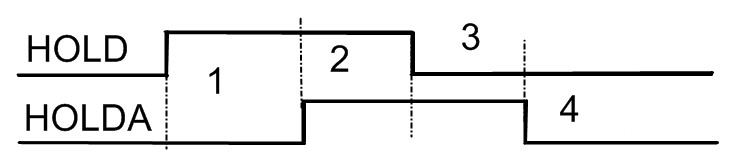
\includegraphics[width=0.75\columnwidth]{img/4waysHandshake}
\caption{Sincronizzazione a quattro fasi}
\label{fig:4waysHandshake}
\end{figure}

In figura \ref{fig:chiComanda} notiamo che l'interfaccia può essere contattata sia dalla CPU (mediante l'opportuno \textit{chip select}, sia dal DMAC tramite il DACK. Grazie al segnale di HOLDA riusciamo discriminare i due casi (ciclo comandato dalla CPU o dal DMAC).

\begin{figure}[!h]
\centering
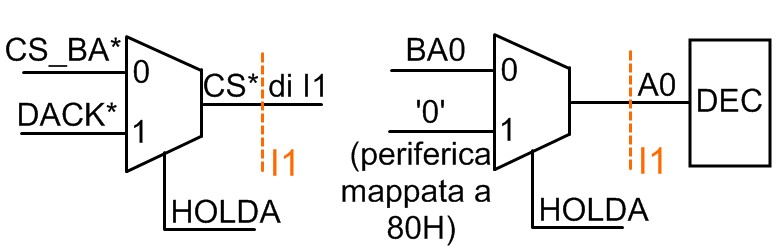
\includegraphics[width=0.75\columnwidth]{img/chiComanda}
\caption{Chi comanda il bus?}
\label{fig:chiComanda}
\end{figure}

\section{\textit{Single mode} vs. \textit{demand mode}}
\label{sec:singleDemand}

In figura \ref{fig:DDSdemandsingle} vediamo, illustrate sotto forma di diagramma degli stati, due modalità di funzionamento del nostro DMAC. 
Nella prima modalità (raffigurata a sinistra) il DMAC è utilizzato in \textit{single mode}: questo significa che, una volta servita la richiesta, il DMAC si pone in IDLE e viene immediatamente restituito il bus alla CPU. In questo caso il DRQ è fisso a 1, il che significa che vi è un continuo rimpallo fra DMA e MICRO (almeno fino a quando HOLD = 0).
Con le modifiche segnate in rosso passiamo invece al \textit{demand mode}: in base a quest'ultima strategia viene dato fiato alla CPU solo alla fine del trasferimento da parte del DMAC. L'efficienza nel trasferimento dei dati è in questo caso maggiore (il continuo rimpallo fra DMAC e CPU genera molto \textit{overhead}), ma c'è rischio di \textit{starvation} per la CPU.
Entrambe le modalità sono supportate dal DMAC.

\begin{figure}[!h]
\centering
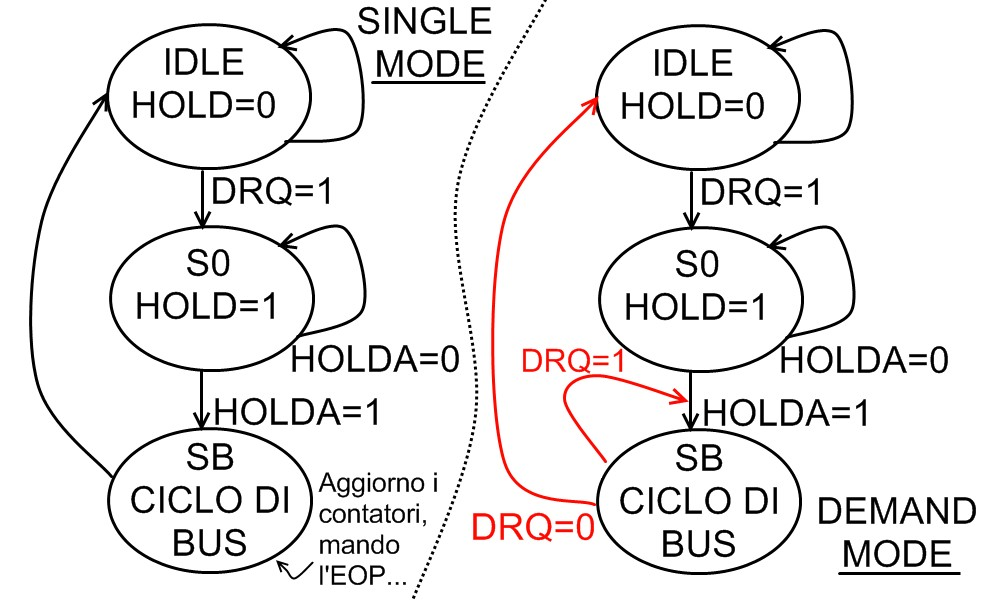
\includegraphics[width=0.75\columnwidth]{img/DDSdemandsingle}
\caption{Diagramma degli stati del \textit{demand mode} e del \textit{single mode}}
\label{fig:DDSdemandsingle}
\end{figure}

\section{Gestione di più periferiche}
\label{sec:gestionePiuPeriferiche}

\begin{figure}[!h]
\centering
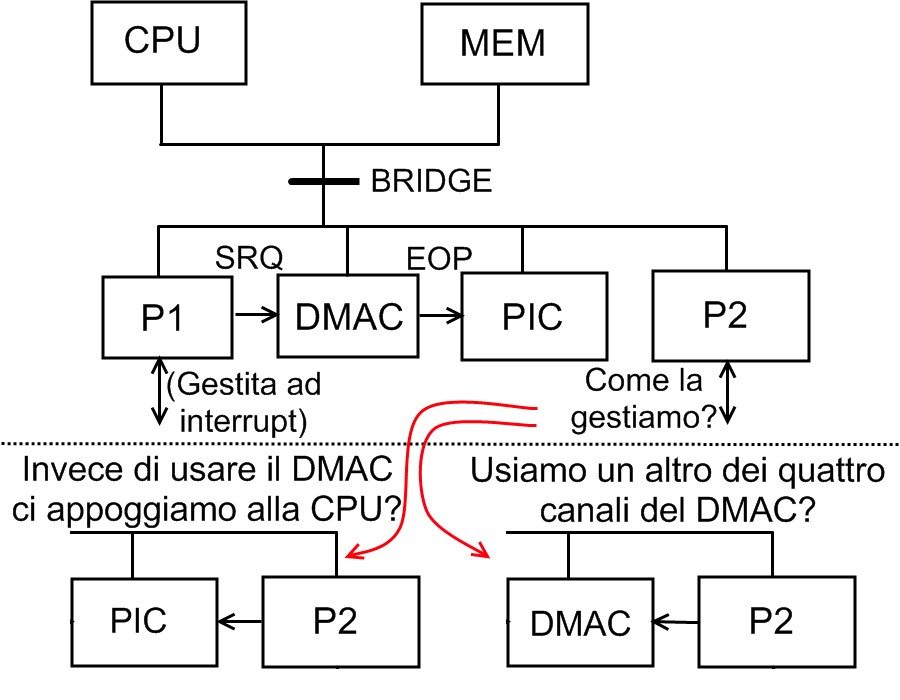
\includegraphics[width=0.75\columnwidth]{img/secondaPeriferica}
\caption{Gestione di più periferiche}
\label{fig:secondaPeriferica}
\end{figure}

In figura \ref{fig:secondaPeriferica} vengono mostrate due possibili scelte per interfacciare una seconda periferica (ad esempio una porta seriale, oppure una stampante) al nostro sistema.
Se in effetti supponessimo di avere quattro stampanti (P1\ldots P4), il DMAC (provvisto di quattro canali) ci permetterebbe di stampare con tutte e quattro contemporaneamente: naturalmente il parallelismo sarebbe solo simulato, in quanto i cicli avvengono intrinsecamente in serie (con una politica a divisione di tempo), tuttavia i tempi di funzionamento della stampante sono molto più lenti di un ciclo di bus quindi l'illusione è quella di un \textit{multitasking} "'puro'".
Chiaramente, con quattro periferiche, abbiamo quattro segnali di SRQ indipendenti fra loro (e asincroni): il DMAC si occupa di gestirli tutti, facendo da arbitro. Inoltre, come già abbiamo sottolineato precedentemente, abbiamo quattro coppie di registri (CAR, CCR), una per ogni canale. 
Nel caso di più di una periferica possono perciò essere fatte delle piccole modifiche per il diagramma degli stati in figura \ref{fig:DDSdemandsingle}: il risultato è mostrato in figura.

\begin{figure}[!h]
\centering
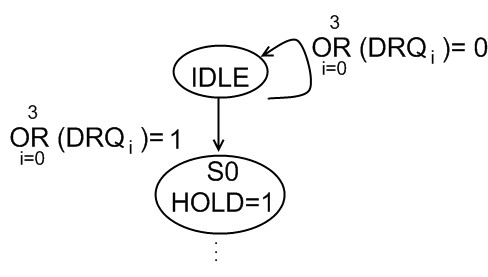
\includegraphics[width=0.55\columnwidth]{img/modifica3periferiche}
\caption{Diagramma degli stati nel caso di quattro periferiche}
\label{fig:modifica3periferiche}
\end{figure}

Anche in questo caso si parla di \textit{single mode} e \textit{demand mode}, con modalità assolutamente analoghe a quelle già viste nel paragrafo \ref{sec:singleDemand}.


%\clearpage

\section{Interfaccia del DMAC, più in dettaglio}
\label{sec:interfacciaDMACDettaglio}

\begin{figure}[!h]
\centering
\includegraphics[width=0.45\columnwidth]{img/piediniDMAC}
\caption{Interfaccia del DMAC, più in dettaglio}
\label{fig:piediniDMAC}
\end{figure}

In questo paragrafo ci occupiamo di esaminare un po' più in dettaglio l'interfaccia del DMAC, che viene mostrata in figura \ref{fig:piediniDMAC}.


A destra vi sono tutti segnali dei quali abbiamo già parlato: vi è una coppia (DREQ, DACK\footnote{In caso di più periferiche è il DACK attivo a segnalarci quella che ha scatenato l'evento da trattare.}) per ogni periferica e un EOP* che si attiva tutte le volte che il $CCR=-1$. Questo segnale viene dato come bidirezionale in quanto si ha sia comunicazione dalla periferica al DMAC (con il segnale EOM, \textit{End Of Message}, che serve a forzare la fine della transazione dall'esterno ponendo il bit di stato TC, \textit{Terminal Count}\footnote{Ve n'è uno per canale e indica che il conteggio è giunto al termine. Viene calcolato facendo l'AND di tutti i bit del \textit{Current Counter Register}: tale operazione darà risultato 1 solo se tutti i bit del CCR saranno pari ad 1, ovvero se codificano il numero -1.} pari ad 1) sia dal DMAC al PIC.


A sinistra abbiamo invece i segnali IORD* e MEMWR* (attivi durante i cicli \textit{fly-by}), IOWR* e MEMRD* (attivi se stiamo scrivendo sulla periferica)\footnote{Si noti che IORD* e IOWR* sono bidirezionali in quanto il DMAC è indirizzabile dal microprocessore in quanto può configurarsi come \textit{slave} (in particolare quando è IDLE) per la trasmissione di dati verso le periferiche.}.
D[0\ldots 7] è la porta dati (posseduta da ogni dispositivo \textit{slave}).
I piedini A[0\ldots 3] servono ad indirizzare i 16 registri all'interno del DMAC (che è una periferica con $K=4$), mentre il segnale READY serve nei frangenti in cui il DMAC è \textit{master} per far gestire correttamente a quest'ultimo i cicli di bus. Gli altri piedini A[4\ldots 7] non sono bidirezionali ma sono soltanto in uscita e vengono accoppiati ai piedini D[0\ldots 7], i quali sono multiplexati per poter funzionare sia come porta dati (come descritto sopra) sia come porta per fornire gli 8 bit più significativi dell'indirizzo da 16 bit in grado di puntare ai famosi 64 KB di I/O (vedi figura \ref{fig:comeFare16bit}). ADSTB Si attiva solo nello stato T1 del ciclo di bus e serve a \textit{latchare} la parte alta dell'indirizzo (piedini D).

\begin{figure}[!h]
\centering
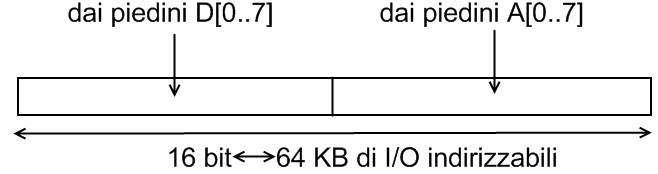
\includegraphics[width=0.55\columnwidth]{img/comeFare16bit}
\caption{Come vengono ottenuti i 16 bit per l'indirizzamento in I/O}
\label{fig:comeFare16bit}
\end{figure}

Infine, per controllare uno spazio di indirizzamento di 4GB (il DMAC accede alla memoria!), è necessario estendere il bus degli indirizzi in modo da consentire la generazione di BA[31\ldots 16]; a tal fine si utilizzeranno appositi registri esterni (\textit{latch}, comandati da HOLDA) per ciascun canale (vedi fig. \ref{fig:altriBit}). 

\begin{figure}[!h]
\centering
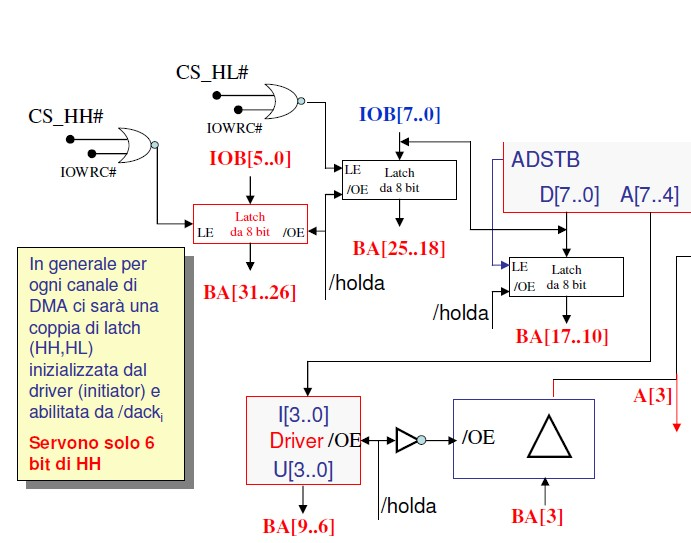
\includegraphics[width=0.75\columnwidth]{img/altriBit}
\caption{Come vengono generati gli altri bit per indirizzare la memoria.}
\label{fig:altriBit}
\end{figure}

AEN, altro piedino, possiamo dimenticarcelo in quanto è un clone di HOLDA. 

Si noti che:
\begin{itemize}
\item nei trasferimenti singoli viene sempre generato il byte più significativo dell'indirizzo (stato T1 dei quattro stati del ciclo di bus);
\item nei trasferimenti \textit{burst}, dopo il primo trasferimento, i successivi includono lo stato T1 solo se
varia il byte più significativo dell'indirizzo.
\item quando il DMAC è utilizzato per spostare dati all'interno della RAM (Memory-to-Memory) si hanno trasferimenti \textit{burst}, ma il byte più significativo dell'indirizzo viene generato in
tutti i trasferimenti. Inoltre ho bisogno di 2 indirizzi e di 2 CCR (uno per l'indirizzo di "'partenza'" e l'altro per l'indirizzo di "'arrivo'"), ma di 1 solo CAR. Inoltre è necessario disporre un registro temporaneo TEMP in quanto è impossibile effettuare un trasferimento MEM-to-MEM in maniera \textit{fly-by}: le memorie, infatti, non possono essere contemporaneamente lette e scritte.
\end{itemize}

\section{Altri due modi di funzionamento: \textit{cascade} e \textit{block}}
\label{sec:altriDueModi}

Il \textit{block mode} è da usare con molta cautela: se attivato, a fronte di una richiesta il DMAC si
impossessa del bus ed esegue \emph{tutti} i trasferimenti previsti dal programma di canale prima di rilasciare il
bus (il diagramma a stati, in pratica, si modifica mantenendo il trasferimento finché il \textit{terminal count} TC è pari a 0 e tornando ad IDLE, con il conseguente rilascio del bus, solo quando TC passa al valore logico alto). Questa modalità è potenzialmente criminale in quanto sprechiamo moltissimi cicli di clock se la periferica è lenta, inoltre il DMA - non essendo sincronizzato con la periferica - parte "'a busso'" (cit.) e duplica dati in virtù del fatto che questi ultimi tardano ad aggiornarsi. Il \textit{block mode} si adatta bene al\textit{ memory-to-memory transfer}\footnote{Ad esempio è possibile effettuare una somma $C=A+B$ fra locazioni interne alla RAM.}, tanto quando il DMA è \textit{master} ha la capacità di pilotare il bus degli indirizzi.

In \textit{cascade mode}, invece, ai pin DREQ/DACK vengono collegati i pin HOLD/HOLDA di un altro dispositivo DMAC. Un DMAC in \textit{cascade mode} non genera il ciclo \textit{fly-by} e si interfaccia con analoghi componenti che considereremo di livello gerarchico inferiore (vedi fig. \ref{fig:cascade}). In questo modo è possibile gestire più di quattro periferiche.

\begin{figure}[!h]
\centering
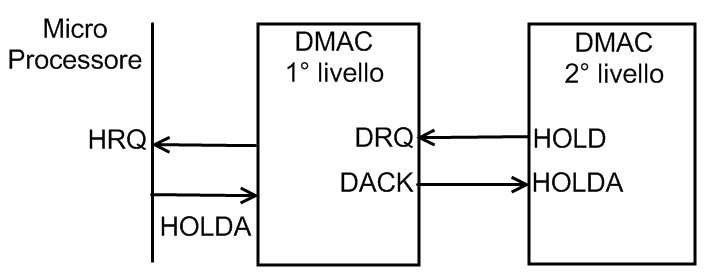
\includegraphics[width=0.55\columnwidth]{img/cascade}
\caption{Interfacciamento dei DMAC in \textit{Cascade Mode}}
\label{fig:cascade}
\end{figure}

In figura \ref{fig:dmacIndirizzi} viene mostrato l'interfacciamento del DMAC per la gestione degli indirizzi (con particolare rilievo per ciò che riguarda la gestione dei segnali di \textit{bank enable}): se "'saliamo'" verso l'alto il microprocessore sta controllando il DMCA, se invece scendiamo è il DMAC ad essere il master.

\begin{figure}[!h]
\centering
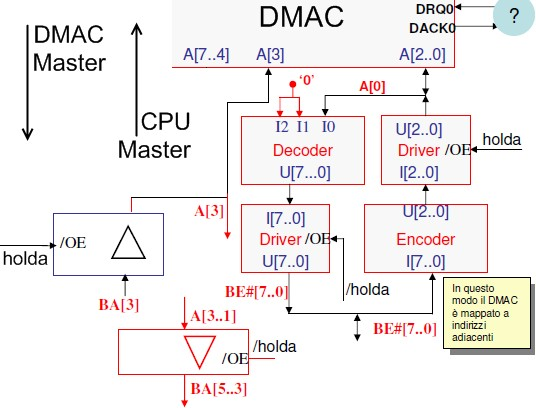
\includegraphics[width=0.75\columnwidth]{img/dmacIndirizzi}
\caption{Interfacciamento del DMAC per la gestione degli indirizzi}
\label{fig:dmacIndirizzi}
\end{figure}

\section{Modalità autoinizializzante}
\label{sec:autoinit}

Esiste una modalità (autoinizializzazione) in cui il DMAC è in grado di settare (inizializzare) correttamente i registri CAR e CCR senza interpellare il microprocessore, fatta l'ipotesi che la serie di operazioni da compiere contenga istruzioni tutte simili fra loro. Esistono infatti due registri "'copia'", chiamati BAR e BCR, i quali contengono rispettivamente una copia dei valori iniziali del CAR e del CCR per il nostro trasferimento. I registri BAR e BCR sono di tipo \textit{write-only}: non dovremo infatti mai andare a leggerne il contenuto, mentre dovremo aggiornarli nel caso i CAR/CCR iniziali dovessero cambiare a seguito di una diversa operazione da compiere. Per fare sì che i valori vengano correttamente settati all'inizio di ogni serie di transizioni, l'indirizzo di BAR e BCR viene fatto coincidere con quello di CAR e CCR (tanto l'ambiguità viene risolta dal fatto che CAR e CCR sono \textit{read-write}, mentre BAR e BCR sono "'blindati'" in quanto \textit{write-only}: quando si va a leggere, quindi, vengono automaticamente restituiti CAR e CCR).

Quando il microprocessore è \textit{master} comanda il DMAC tremite istruzioni a 8 bit (che l'ormai noto parallelismo del bus di I/O); come possiamo allora trasferire i 16 bit al BAR? Sicuramente serviranno due OUT, ma non sarà necessario utilizzare due diversi indirizzi per distinguerne le due parti (più o meno significativa). Infatti è presente, nel \textit{chip select} di questi due registri, una funziona combinatoria che in base ai bit BA distingue quale fra i quattro canali del DMAC è interessato e seleziona la parte più o meno significativa del BAR utilizzando un bit generato da un \textit{first-last flip-flop} che commuta di continuo tra '0' e '1'. Tale \textit{flip-flop} viene resettato a '0' con il comando \textit{clear first-last} ed è in grado di selezionare distintamente prima la parte meno significativa e poi l'altra senza bisogno della generazione distinta dei due indirizzi.

\clearpage
\section{Forme d'onda}
\label{sec:formeOnda}

\begin{figure}[!h]
\centering
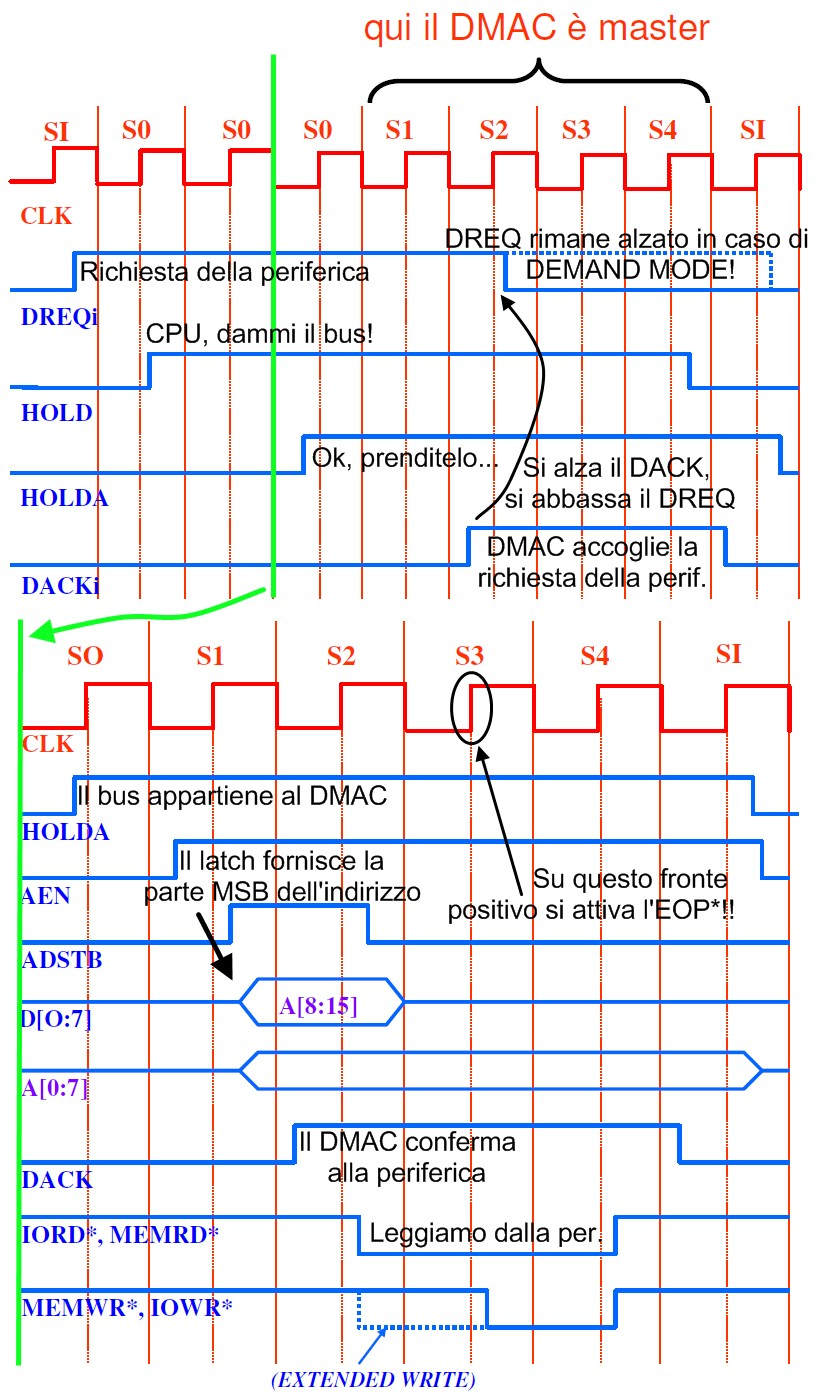
\includegraphics[width=0.78\columnwidth]{img/OndeDMAC}
\caption{Forme d'onda dei segnali del DMAC}
\label{fig:OndeDMAC}
\end{figure}

%\section{Appendice: periferica a 16 bit}
%\label{sec:periferica16}
%
%In figura \ref{fig:periferica16} vediamo una versione a 16 bit della periferica mostrata nel paragrafo \ref{sec:transazioniIO}.
%
%\begin{figure}[!h]
%\centering
%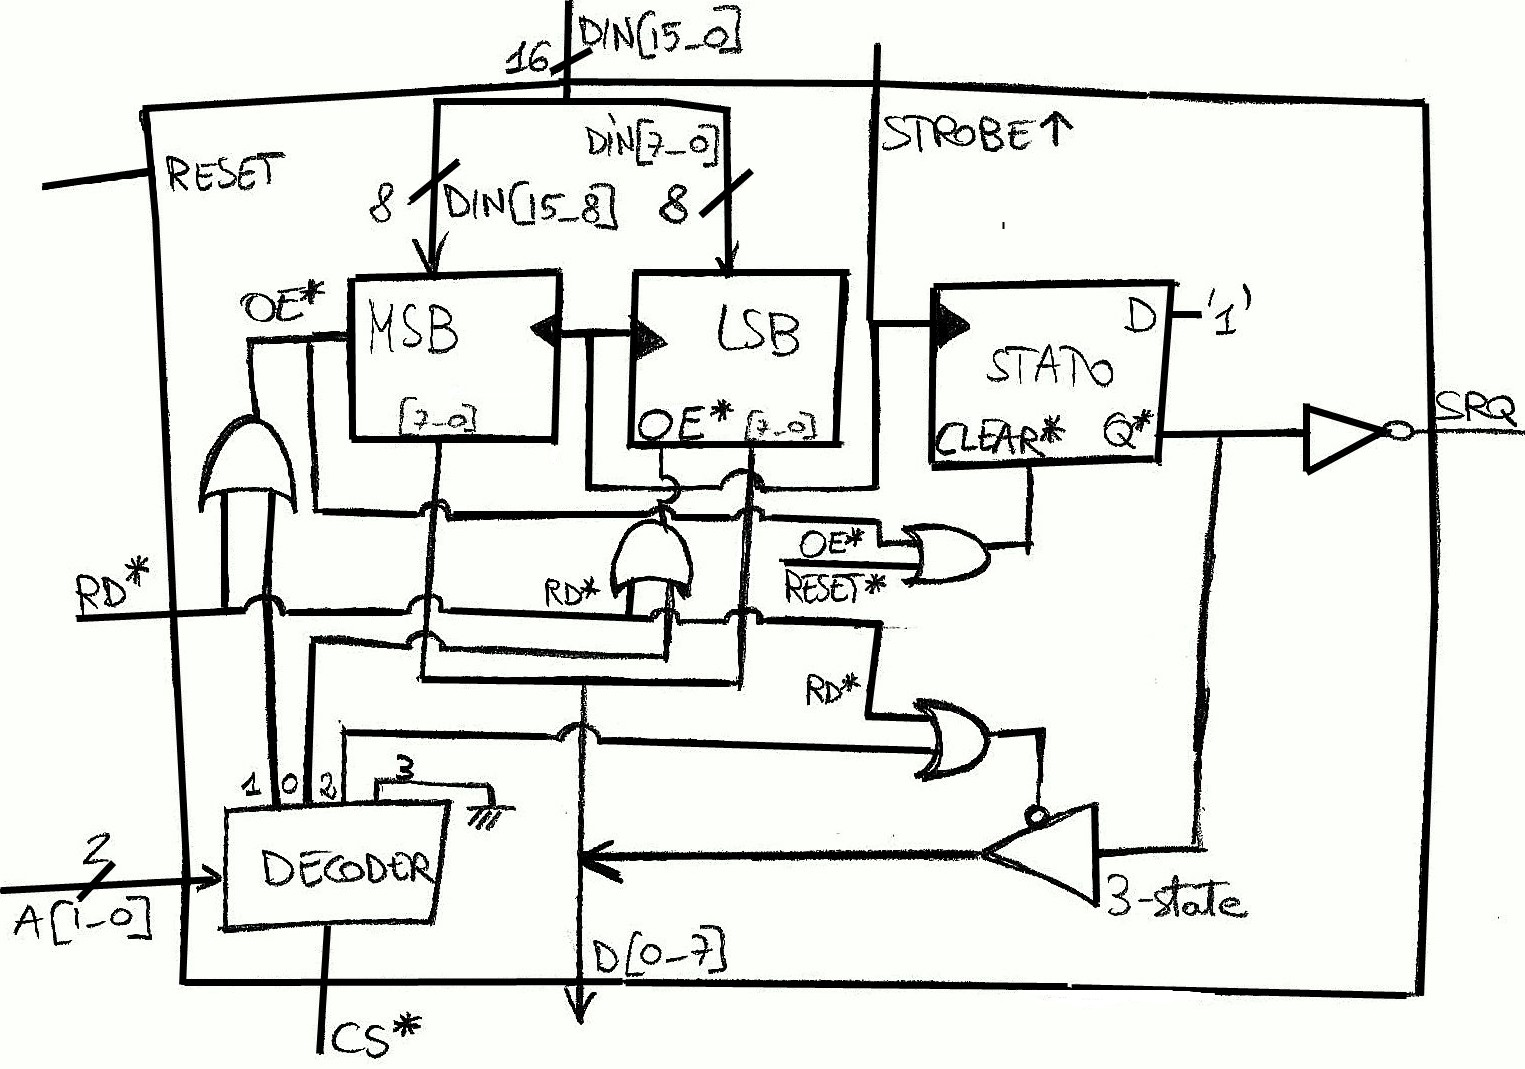
\includegraphics[width=0.85\columnwidth]{img/periferica16}
%\caption{Periferica a 16 bit}
%\label{fig:periferica16}
%\end{figure}

